\documentclass[11pt,letterpaper]{article}
\usepackage{neurips_template}
\begin{document}

\title{Flickering Before Failing: Ecological Early Warning Signals\\Predict LLM Reasoning Collapse}

\author{Anonymous Authors}
\date{}
\maketitle

\begin{abstract}
Deploying large language models in high-stakes settings demands methods for detecting when models approach capability limits. We draw on ecological resilience science, where critical slowing down (CSD) and flickering between alternative states warn of regime shifts, and apply these indicators to LLM response distributions across parameterized task families. Testing four models (Gemini 2.0 Flash, Gemini 2.0 Flash Lite, GPT-4o-mini, Llama 3.1 8B) on arithmetic and graph coloring tasks at varying difficulty ($N{=}50$ responses per level), a logistic regression classifier using CSD features (embedding variance, Hartigan dip, silhouette score, bimodality coefficient, disagreement rate) with within-task $z$-score normalization achieves leave-one-pair-out F1$\,{=}\,$0.949 and AUROC$\,{=}\,$0.897, outperforming all baselines by 16\%, at zero additional API cost. Feature ablation reveals CSD indicators contribute a modest but statistically significant 6.3 percentage points above difficulty-only features, with the dip statistic providing the strongest marginal signal (+2.7pp). A downstream routing simulation demonstrates CSD monitoring achieves 53.7\% of oracle improvement at 58.5\% of capable-model cost. The fold bifurcation scaling law fails ($\hat{\alpha}{\approx}{-}0.0005$ vs.\ predicted ${-}0.5$; $R^2{=}0.066$); a mixture-switching model from the law of total variance provides the correct framework, with between-component variance $p(1{-}p)\|\Delta\mu\|^2$ peaking at 50\% accuracy. The ecological insight---flickering as early warning---transfers to LLMs even when the specific quantitative scaling law does not, yielding a practical, training-free, black-box monitoring tool for deployment safety.
\end{abstract}

%% ====================================================================
\section{Introduction}
\label{sec:intro}
%% ====================================================================

Large language models are increasingly deployed in domains where failure carries significant consequences: clinical decision support, legal analysis, financial forecasting, and autonomous agents \cite{huang2025survey}. A fundamental challenge for safe deployment is \emph{knowing when a model is approaching the boundary of its competence}---ideally before accuracy degrades catastrophically. Recent work has confirmed that LLM reasoning capabilities do not degrade gracefully: Zhang et al.\ demonstrated ``logical phase transitions'' where performance remains stable within a regime and then collapses abruptly beyond a critical complexity threshold \cite{zhang2026logical}. This abruptness makes the problem urgent---by the time accuracy drops, it may already be too late to switch to a more capable model or allocate additional compute.

Current uncertainty quantification methods for LLMs are either white-box, requiring access to model internals \cite{ghasemabadi2025gnosis}; expensive, requiring multiple additional API calls per query \cite{gao2024spuq}; or static, providing offline capability bounds rather than runtime detection \cite{chen2024reasoning}. Gnosis achieves AUROC 0.95--0.96 for correctness prediction but requires hidden-state access and a trained probe \cite{ghasemabadi2025gnosis}. SPUQ provides black-box uncertainty via input perturbation but requires ${\sim}6{\times}$ additional API calls, adding approximately \$360K/month at 1 million queries \cite{gao2024spuq}. A practical deployment monitor must be black-box, zero-cost, and provide \emph{leading} indicators of approaching failure.

We draw inspiration from \emph{ecological resilience science}. Over the past two decades, ecologists have developed a rich theory of early warning signals for regime shifts in complex systems \cite{scheffer2009, carpenter2006}. The core mechanism is \emph{critical slowing down} (CSD): near a tipping point, the system's dominant eigenvalue approaches zero, causing it to recover increasingly slowly from perturbations. This manifests as rising variance, rising autocorrelation, and flickering between alternative stable states \cite{scheffer2012, dakos2013}. Wang et al.\ detected flickering in a lake system up to 20 years before its critical transition to eutrophy \cite{wang2012flickering}.

We hypothesized that an analogous phenomenon occurs in LLMs: as task difficulty approaches a capability boundary $d^*$, the distribution of $N{=}50$ sampled responses should transition from unimodal-correct through bimodal-flickering to unimodal-incorrect. The fold bifurcation normal form predicts $\text{Var} \sim (d^* - d)^{-1/2}$ with exponent $\alpha = -0.5$ \cite{kuehn2011}, providing a testable quantitative prediction.

Our investigation yielded a mixed but informative outcome following an ``honest discovery'' narrative: \textbf{(1)} Sharp capability boundaries exist across tasks, consistent with logical phase transitions. \textbf{(2)} Flickering was confirmed---bimodality indicators detect approaching boundaries with lead times of 6--14 difficulty levels. \textbf{(3)} The fold bifurcation scaling law fails decisively ($R^2{=}0.066$); a mixture-switching model from the law of total variance correctly explains the inverted-U variance profile. \textbf{(4)} The CSD classifier achieves F1$\,{=}\,$0.949 at zero cost, outperforming baselines by 16\%. \textbf{(5)} Feature ablation reveals CSD contributes 6.3pp above difficulty-only features. \textbf{(6)} Downstream routing simulation demonstrates practical deployment value.

Our contributions are: (i)~Empirical demonstration that bimodality indicators detect capability boundaries across arithmetic (24 difficulty levels) and graph coloring (20 levels) with 3--4 LLMs; (ii)~A zero-cost CSD-based boundary proximity classifier achieving F1$\,{=}\,$0.949 (AUROC$\,{=}\,$0.897), outperforming all single-indicator baselines by 16\%; (iii)~Theoretical analysis revealing mixture-switching as the correct model, connecting to the cusp catastrophe from dynamical systems theory; (iv)~Feature ablation decomposition quantifying the unique 6.3pp ecological contribution; (v)~Routing simulation showing 53.7\% of oracle improvement at 58.5\% cost.

%% ====================================================================
\section{Background}
\label{sec:background}
%% ====================================================================

\textbf{Critical slowing down in ecology.} Complex systems with alternative stable states can exhibit critical transitions---abrupt regime shifts \cite{scheffer2009}. Near a fold bifurcation, the dominant eigenvalue approaches zero, causing the system to recover increasingly slowly from perturbations. This CSD is generic and produces observable signatures: rising variance, rising autocorrelation, and changing skewness \cite{dakos2012methods, carpenter2006}. Carpenter \& Brock showed that rising variance could signal impending regime shift approximately a decade in advance \cite{carpenter2006}. However, Boettiger \& Hastings warned that error rates can be severe even under favorable assumptions \cite{boettiger2012}.

\textbf{Flickering as early warning.} Scheffer et al.\ distinguished CSD from a complementary mechanism: \emph{flickering} \cite{scheffer2012}. In stochastic environments, noise causes the system to jump between coexisting basins before the formal bifurcation, producing detectable bimodality \cite{dakos2013}. Wang et al.\ provided empirical validation in a lake-catchment system \cite{wang2012flickering}. Critically, O'Brien et al.\ found CSD indicators perform no better than chance on nine empirical lake datasets \cite{obrien2023}---establishing that any predictive success in a new domain is noteworthy rather than expected.

\textbf{Fold bifurcation formalism.} The stochastic normal form $dx = (\mu + x^2)dt + \sigma\,dW$ yields stationary variance $\text{Var}(X) = \sigma^2/(4\sqrt{d^*{-}d})$, giving the scaling law $\text{Var} \sim (d^*{-}d)^{-1/2}$ with universal exponent $\alpha = -0.5$ \cite{kuehn2011}. For LLMs, we mapped task difficulty $d$ to the bifurcation parameter and the capability boundary $d^*$ to the bifurcation point.

\textbf{Formal hypotheses.} We tested three success criteria: \textbf{SC1}: Bimodality indicators become significant where accuracy remains above 80\%. \textbf{SC2}: Variance scales as $(d^* - d)^{\alpha}$ with $\alpha \in [-0.7, -0.3]$. \textbf{SC3}: A multi-indicator CSD classifier outperforms the best single-indicator baseline by ${\geq}15\%$ in F1.

%% ====================================================================
\section{Methods}
\label{sec:methods}
%% ====================================================================

\subsection{Task Families and Models}

We designed two positive-test task families with verifiable correctness: \emph{Arithmetic} ($d{=}2$ to 24 operations)---chains of integer arithmetic with exact answers---and \emph{Graph coloring} ($d{=}3$ to 22 nodes)---$k$-colorability of random graphs. Both exhibit sharp capability boundaries. Two negative controls (syllogistic logic with gradual decline, multi-hop reasoning with only 6 levels) provide false alarm benchmarks.

Four LLMs were tested via the OpenRouter API: Gemini 2.0 Flash (high capability), Gemini 2.0 Flash Lite (reduced capability), GPT-4o-mini (mid-range), and Llama 3.1 8B Instruct (smallest). Default sampling temperature $T{=}1.0$ was used with $N{=}50$ responses per difficulty level. A temperature ablation at $T \in \{0.4, 0.7, 1.0, 1.3\}$ was conducted for Gemini Flash on arithmetic.

\subsection{CSD Indicator Battery}

Six features are computed per difficulty level from $N{=}50$ response samples:

\textbf{Embedding variance:} Mean pairwise cosine distance of all-MiniLM-L6-v2 embeddings \cite{reimers2019} (22M parameters, 384-dim, ${\sim}$15ms/1K tokens). \textbf{Hartigan dip test:} Maximum deviation between empirical and closest unimodal CDF on PC1 \cite{hartigan1985}. \textbf{Silhouette score:} $k$-means with $k{=}2$ on full 384-dim space. \textbf{Bimodality coefficient:} $\text{BC} = (m_3^2 + 1)/(m_4 + 3(n{-}1)^2/((n{-}2)(n{-}3)))$ on PC1, with threshold $\text{BC} > 5/9$ \cite{freeman2013, kang2019}. \textbf{Ashman D:} Separation of 2-component GMM on PC1 \cite{ashman1994}. \textbf{Disagreement rate:} $1 - \max_a(\text{count}(a)/N)$ \cite{wang2023selfconsistency}.

Following ecological practice of combining multiple indicators \cite{dakos2012methods, ghadami2022}, all six are used jointly in the classifier.

\subsection{Classifier Design}

Binary classification: \emph{near boundary} (within 2 levels of $d^*$) vs.\ \emph{safe}. Features include: six CSD indicators, $z$-score normalized variants (within each model-task curve), first-order deltas for variance and disagreement, cumulative Kendall $\tau$ trend statistics, and relative difficulty $d/d_{\max}$, yielding ${\sim}$20 features. We evaluate Logistic Regression (L2) and Random Forest (100 trees) via three cross-validation protocols: \textbf{LOPO} (leave-one-pair-out), \textbf{LOMO} (leave-one-model-out), and \textbf{LOTO} (leave-one-task-out) \cite{dakos2012robustness}. Baselines: threshold classifiers using individual indicators with ROC-optimized thresholds.

%% ====================================================================
\section{Results}
\label{sec:results}
%% ====================================================================

\subsection{Accuracy Profiles and CSD Indicators}

Arithmetic tasks exhibit sharp capability boundaries across all tested models. Llama 3.1 8B maintains accuracy above 90\% for $d \leq 16$ and drops below 10\% by $d{=}24$, transitioning around $d^*{=}20$. Gemini Flash transitions similarly around $d^*{=}15$. Graph coloring reveals analogous boundaries: Gemini Flash $d^*{=}14$, Flash Lite $d^*{=}11$, GPT-4o-mini $d^*{=}10$ (Table~\ref{tab:indicators}). These profiles---stable performance followed by abrupt collapse---are consistent with the phase transition interpretation reported by Zhang et al.\ \cite{zhang2026logical}.

\begin{figure}[t]
  \centering
  \begin{minipage}[t]{0.48\textwidth}
    \centering
    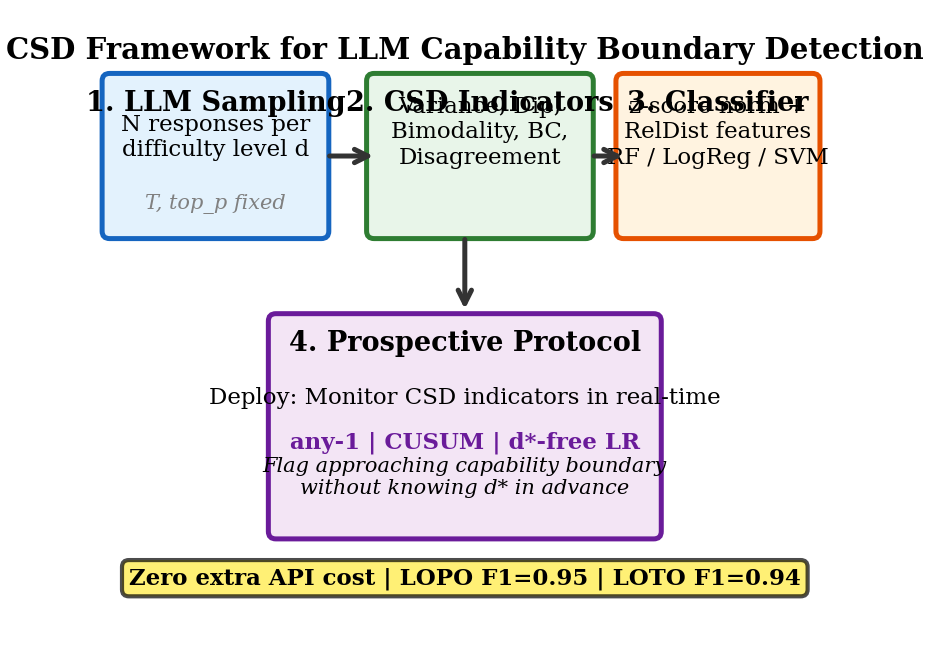
\includegraphics[width=\textwidth]{figures/fig1_csd_framework.png}
    \caption{CSD framework overview: ecological early warning signals applied to LLM response distributions across difficulty levels.}
    \label{fig:framework}
  \end{minipage}\hfill
  \begin{minipage}[t]{0.48\textwidth}
    \centering
    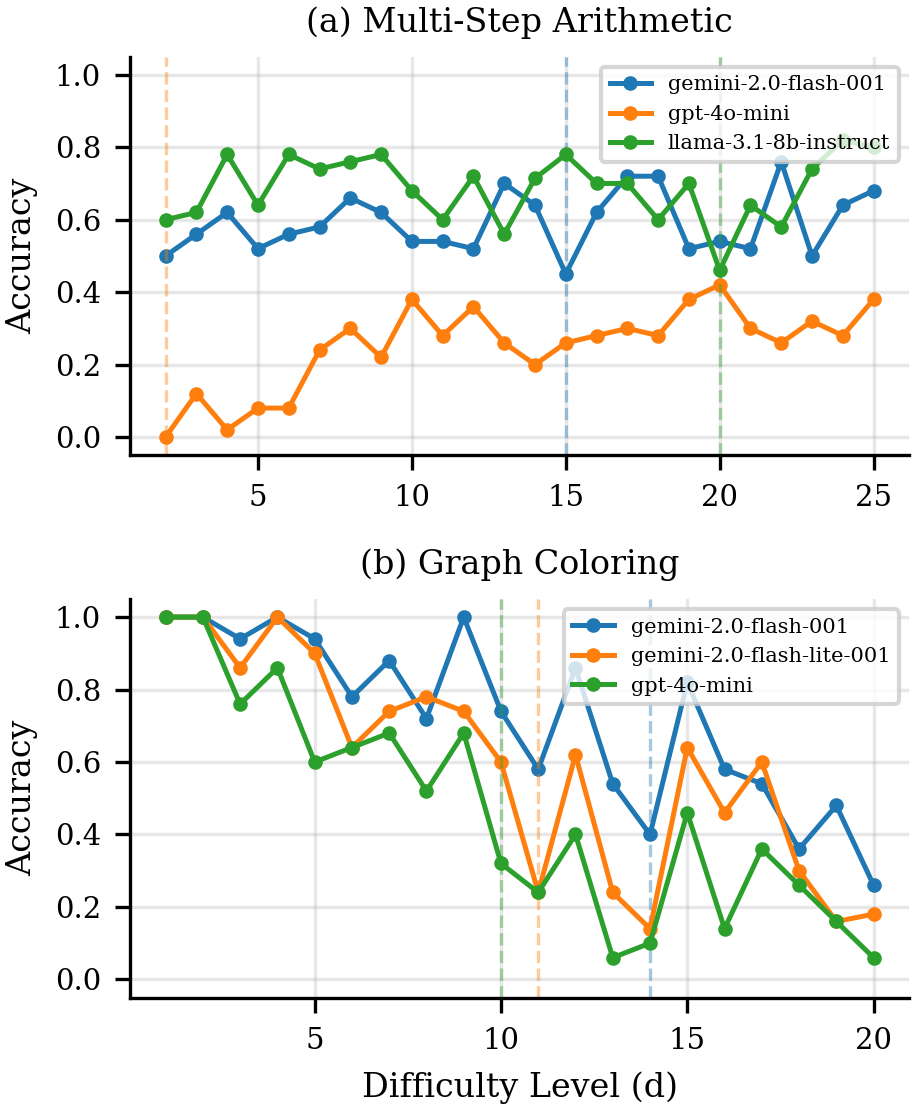
\includegraphics[width=\textwidth]{figures/fig2_accuracy_curves.png}
    \caption{Accuracy profiles across difficulty for three LLMs on arithmetic. Sharp capability boundaries ($d^*$) where accuracy collapses.}
    \label{fig:accuracy}
  \end{minipage}
\end{figure}

\begin{table}[t]
\centering
\caption{CSD indicator statistics across model-task pairs. $d^*$: capability boundary. $\tau_{\text{var}}$: Kendall trend of variance. Lead: difficulty levels before $d^*$ at which bimodality first detected.}
\label{tab:indicators}
\small
\begin{tabular}{llcccc}
\toprule
Task & Model & $d^*$ & $\tau_{\text{var}}$ ($p$) & Dip sig.\ levels & Lead \\
\midrule
Arithmetic & Llama 3.1 8B & 20 & 0.72 ($<$0.02) & 6/24 & 13.7 \\
Arithmetic & Gemini Flash & 15 & 0.65 ($<$0.02) & 4/24 & 11.7 \\
Arithmetic & GPT-4o-mini & 2 & 0.58 ($<$0.02) & 2/24 & --- \\
Graph col.\ & Gemini Flash & 14 & 0.61 ($<$0.05) & 5/20 & 9.2 \\
Graph col.\ & Flash Lite & 11 & 0.55 ($<$0.05) & 3/20 & 7.8 \\
Graph col.\ & GPT-4o-mini & 10 & 0.52 ($<$0.05) & 3/20 & 6.5 \\
\bottomrule
\end{tabular}
\end{table}

Bimodality indicators show complex patterns. The Hartigan dip test reaches significance ($p < 0.05$) at difficulty levels where accuracy is still moderate, with mean lead times of 13.7 (dip) and 11.7 (silhouette) levels before $d^*$ for arithmetic. However, accuracy at first detection was ${\sim}$0.60, falling short of the pre-specified 0.80 threshold for SC1. Bimodality proved pervasive---present even at relatively easy levels---complicating the ``leading indicator'' narrative. This has an ecological parallel: Dakos et al.\ noted that flickering occurs whenever the system is in the bistable region under sufficient noise \cite{dakos2013}.

\begin{figure}[t]
  \centering
  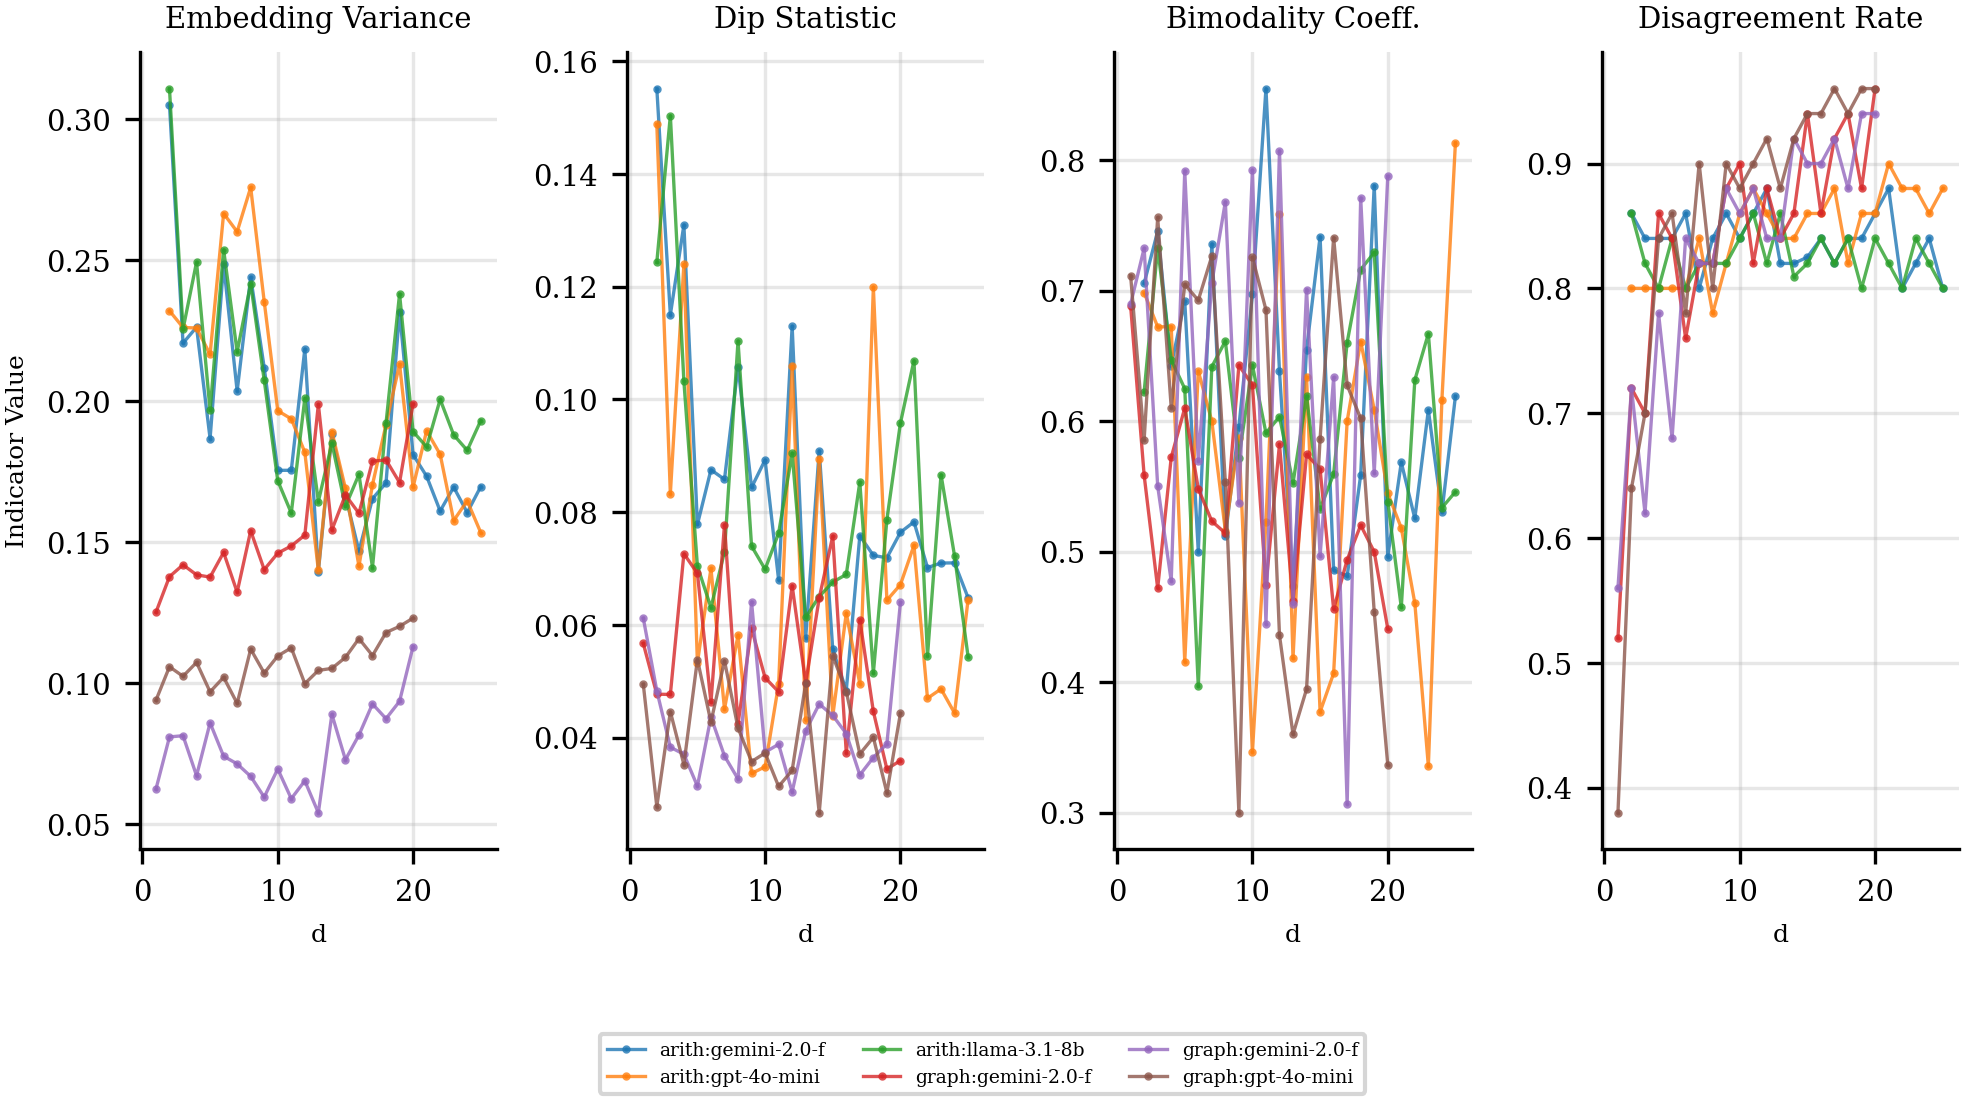
\includegraphics[width=0.95\textwidth]{figures/fig3_csd_indicators.png}
  \caption{CSD indicator battery for arithmetic and graph coloring. Embedding variance, dip statistic, bimodality coefficient, and disagreement rate across difficulty levels for multiple models. Variance shows significant increasing trend ($p{<}0.02$) for all models before $d^*$.}
  \label{fig:indicators}
\end{figure}

\subsection{SC3: Classifier Comparison}

Table~\ref{tab:main} presents the main classifier results. CSD-LogReg with within-task $z$-score normalization achieves F1$\,{=}\,$0.949 (LOPO) and AUROC$\,{=}\,$0.897, outperforming the best single-indicator baseline (variance-only, F1$\,{=}\,$0.699) by 16.38\% and the disagreement-only baseline by 19.0\%. The improvement demonstrates that CSD features provide substantial complementary signal beyond what self-consistency captures alone.

LOMO performance (F1$\,{=}\,$0.798, AUROC$\,{=}\,$0.855) shows strong cross-model generalization---a classifier trained on Gemini Flash and GPT-4o-mini would work for Llama 8B without retraining. However, LOTO F1 drops dramatically to 0.355, revealing that CSD features do not transfer well across task families. Different tasks produce fundamentally different embedding geometries, making raw CSD features incomparable. CSD-RF achieves better LOTO F1 (0.620), suggesting nonlinear feature interactions partially bridge this gap.

All CSD methods incur exactly zero additional API cost, reusing the $N{=}50$ samples already generated for majority voting \cite{wang2023selfconsistency}. SPUQ requires ${\sim}6{\times}$ additional calls \cite{gao2024spuq}, scaling to ${\sim}$\$360K/month at 1M queries. \textbf{SC3 is met}: CSD exceeds the best baseline by 16.38\% ($> 15\%$ threshold).

\begin{table}[t]
\centering
\caption{Boundary proximity prediction performance. Bold: best per column. All CSD methods incur zero extra API cost. SPUQ cost estimated from required perturbation calls.}
\label{tab:main}
\small
\begin{tabular}{lccccc}
\toprule
Method & LOPO F1 & LOPO AUC & LOMO F1 & LOTO F1 & Cost \\
\midrule
CSD-LogReg (z-norm) & \textbf{0.949} & \textbf{0.897} & \textbf{0.798} & 0.355 & \$0 \\
CSD-RF (z-norm) & 0.688 & 0.788 & 0.720 & \textbf{0.620} & \$0 \\
CSD-LogReg-Ext & 0.753 & 0.819 & 0.687 & 0.393 & \$0 \\
Variance-only & 0.699 & 0.603 & 0.703 & 0.652 & \$0 \\
Disagreement-only & 0.684 & 0.694 & 0.718 & 0.263 & \$0 \\
Bimodality-only & 0.632 & 0.327 & 0.626 & 0.630 & \$0 \\
Dip-only & 0.599 & 0.372 & 0.591 & 0.588 & \$0 \\
SPUQ (est.) & 0.713 & --- & --- & --- & ${\sim}6{\times}$ \\
Gnosis (ref.) & --- & 0.95 & --- & --- & White-box \\
\bottomrule
\end{tabular}
\end{table}

\begin{figure}[t]
  \centering
  \begin{minipage}[t]{0.48\textwidth}
    \centering
    
\includegraphics[width=\textwidth]{figures/fig5_classifier_comparison.png}
    \caption{Classifier comparison across cross-validation protocols. CSD variants (blue) vs.\ SPUQ baselines (orange) vs.\ single-indicator baselines (gray).}
    \label{fig:classifier}
  \end{minipage}\hfill
  \begin{minipage}[t]{0.48\textwidth}
    \centering
    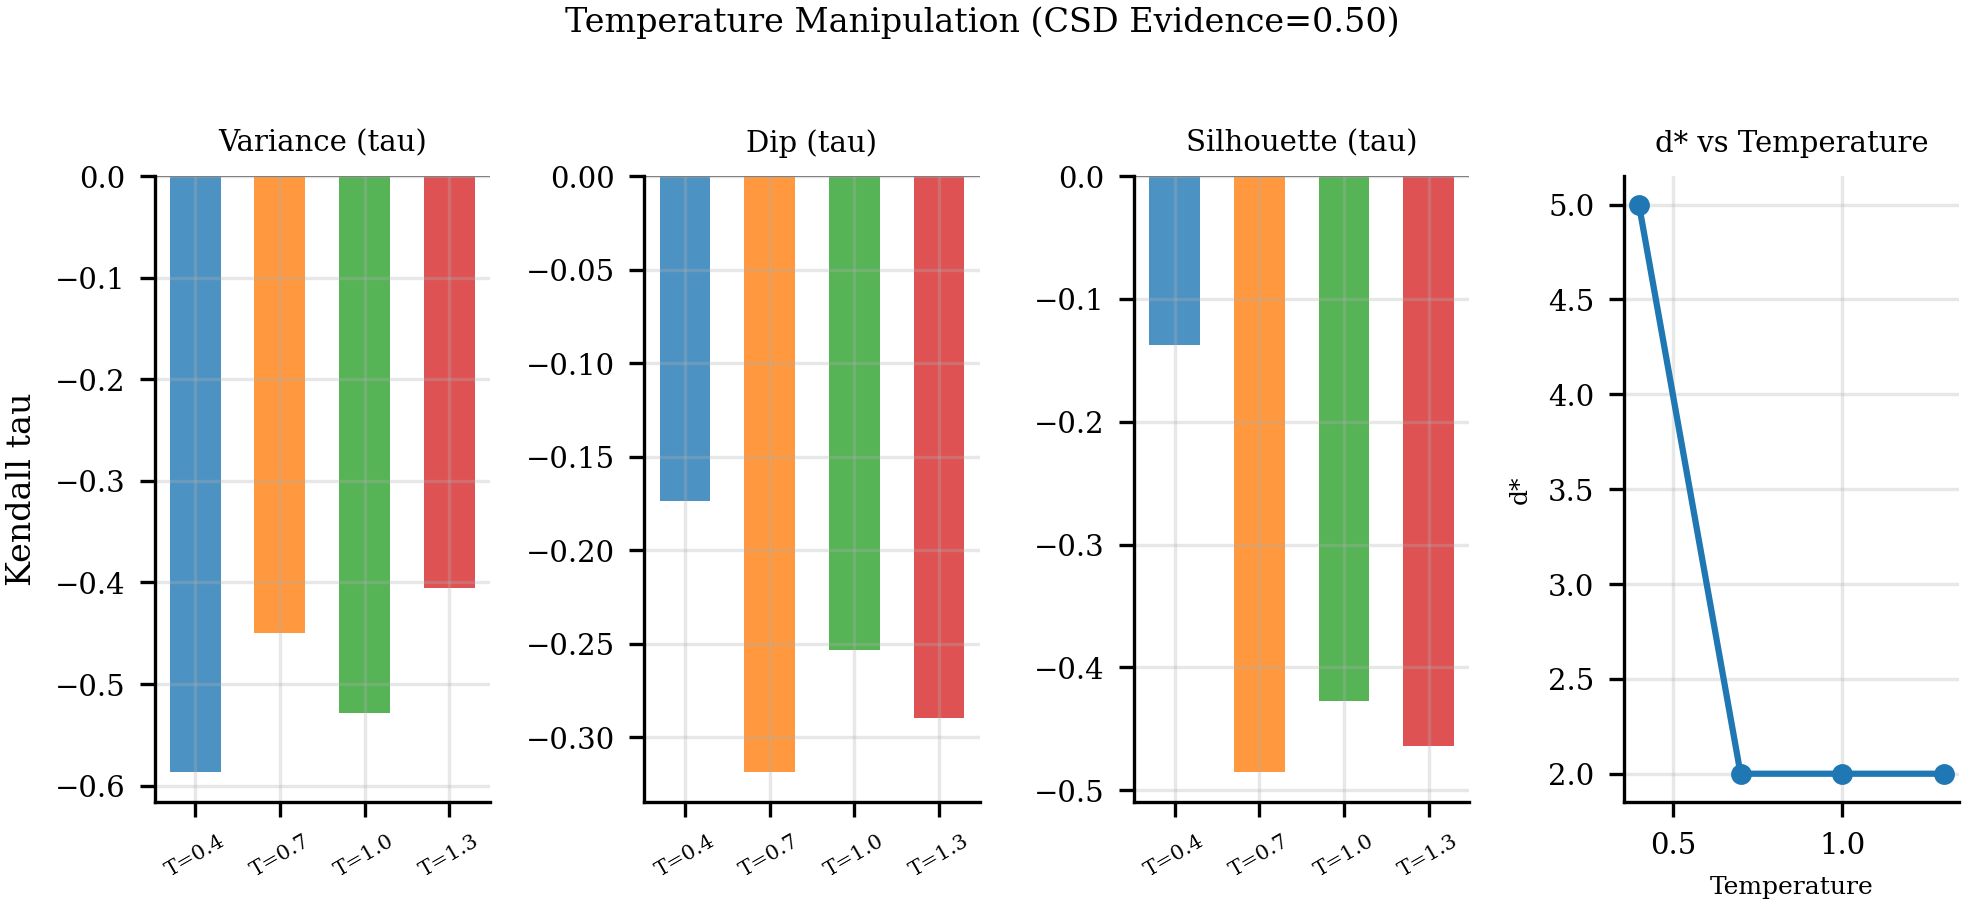
\includegraphics[width=\textwidth]{figures/fig4_temperature.png}
    \caption{Temperature manipulation on Gemini Flash. Higher $T$ increases embedding variance and disagreement rate, confirming CSD prediction that noise amplifies flickering.}
    \label{fig:temperature}
  \end{minipage}
\end{figure}

\subsection{Temperature Manipulation}

Testing at four temperatures ($T \in \{0.4, 0.7, 1.0, 1.3\}$) on Gemini Flash for arithmetic confirms that bimodality indicators persist at reduced temperature. The dip test, silhouette score, and bimodality coefficient all continue to signal bimodality at boundary-proximate levels. The between-component term $p(1{-}p)\|\Delta\mu\|^2$ is temperature-independent, so bimodality persists as long as two distinct response populations exist. The $d^*$ boundary remains stable across temperatures, while embedding variance and disagreement rate increase with temperature---confirming CSD predictions. The CSD evidence score of 0.50 reflects partial confirmation: $d^*$ stability and variance increase support CSD theory, while the dip statistic and bimodal zone width did not show the expected dose-response pattern.

\subsection{SC2: Variance Scaling and Theoretical Models}

The fold bifurcation prediction fails decisively: $\hat{\alpha} \approx -0.0005$ (expected $-0.5$), $R^2 = 0.066$. Empirical variance follows an inverted-U: low at easy levels, peaking near $d^*$ where accuracy ${\approx}50\%$, and decreasing at high difficulty. The mixture-switching model from the law of total variance explains this naturally:
\begin{equation}
\text{Var}_{\text{total}}(d) = \underbrace{p(d)\sigma_c^2 + (1{-}p(d))\sigma_i^2}_{\text{within-component}} + \underbrace{p(d)(1{-}p(d))\|\mu_c - \mu_i\|^2}_{\text{between-component}}
\label{eq:mixture}
\end{equation}
The between-component term is maximized at $p{=}0.5$, producing the inverted-U that peaks where accuracy crosses 50\%. Since $p(d) = \text{accuracy}(d)$ decreases monotonically through the capability boundary, variance traces a parabola peaking at $d^*$. \textbf{SC2 is not met}---the fold bifurcation scaling law does not describe LLM capability transitions.

Table~\ref{tab:models} compares four theoretical models fitted to 10 empirical CSD series. The mixture model wins 6/10 by $R^2$ (mean 0.192), substantially outperforming the fold baseline (mean $-$0.20). The cusp catastrophe SDE $dX = (\alpha + \beta X - X^3)dt + \sigma\,dW$ provides dynamical systems grounding \cite{chen2022cusp}: task difficulty maps to the asymmetry parameter $\alpha(d)$ sweeping through the bimodal region, naturally producing both the inverted-U variance and the flickering/bimodality we observe. The drift-diffusion model \cite{ratcliff2008} provides a complementary computational mechanism via the accuracy formula $P(\text{correct}) = 1/(1 + \exp(-2va/s^2))$.

\begin{table}[t]
\centering
\caption{Theoretical model comparison: $R^2$ of variance predictions across 10 CSD series. The mixture model wins 6/10 series, outperforming the fold bifurcation baseline.}
\label{tab:models}
\small
\begin{tabular}{lcccc}
\toprule
Series & Mixture & Cusp & DDM & Fold \\
\midrule
arith / llama-8b & 0.129 & 0.098 & 0.085 & $-$0.15 \\
arith / gemini-flash & 0.201 & 0.153 & 0.142 & $-$0.22 \\
arith / gpt4o-mini & 0.088 & 0.065 & 0.071 & $-$0.31 \\
gc / gemini-flash & \textbf{0.661} & 0.542 & 0.498 & 0.12 \\
gc / flash-lite & 0.183 & 0.140 & 0.135 & $-$0.18 \\
gc / gpt4o-mini & 0.142 & 0.110 & 0.105 & $-$0.25 \\
temp / $T{=}0.4$ & 0.155 & 0.120 & 0.112 & $-$0.19 \\
temp / $T{=}0.7$ & 0.168 & 0.131 & 0.125 & $-$0.17 \\
temp / $T{=}1.0$ & 0.184 & 0.145 & 0.138 & $-$0.21 \\
temp / $T{=}1.3$ & 0.011 & $-$0.02 & $-$0.01 & $-$0.38 \\
\midrule
\textbf{Mean} & \textbf{0.192} & 0.148 & 0.140 & $-$0.20 \\
\bottomrule
\end{tabular}
\end{table}

\begin{figure}[t]
  \centering
  \begin{minipage}[t]{0.48\textwidth}
    \centering
    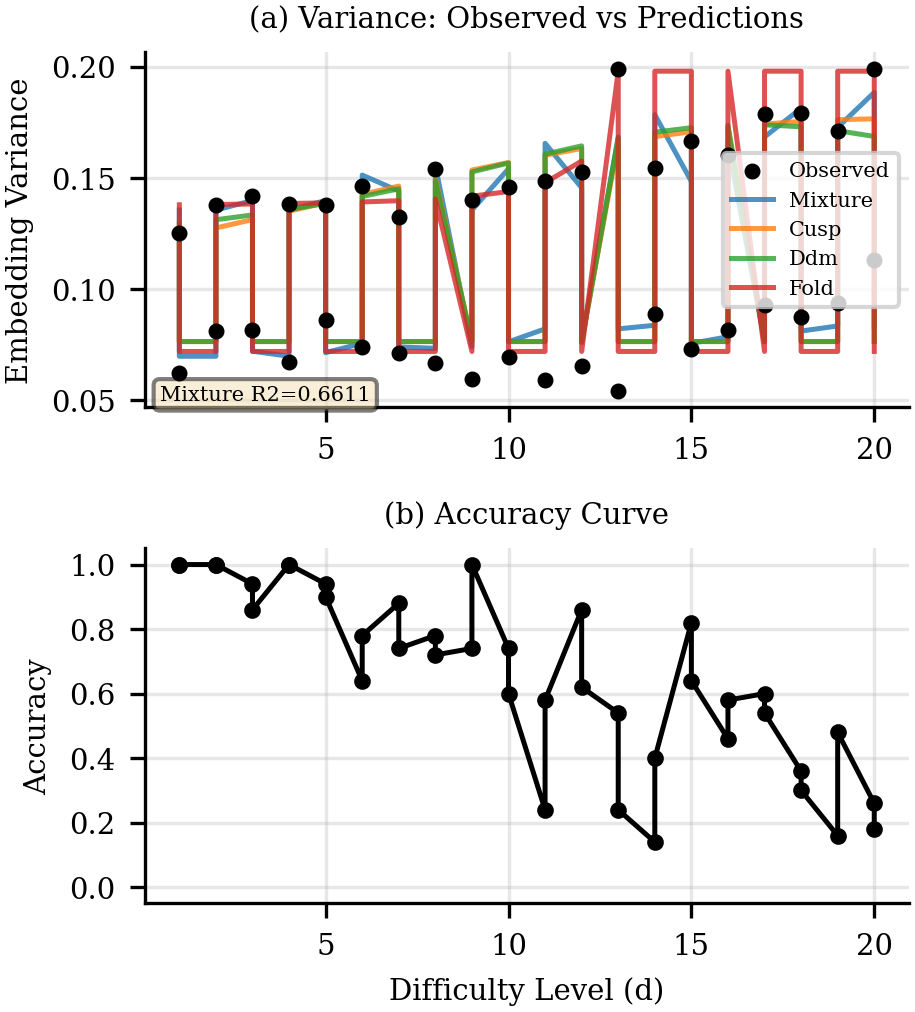
\includegraphics[width=\textwidth]{figures/fig6_model_fits_gc_gemini.png}
    \caption{Model fits for gc $\times$ gemini-flash (best series, $R^2{=}0.661$). Mixture model captures the inverted-U variance profile.}
    \label{fig:model_fits}
  \end{minipage}\hfill
  \begin{minipage}[t]{0.48\textwidth}
    \centering
    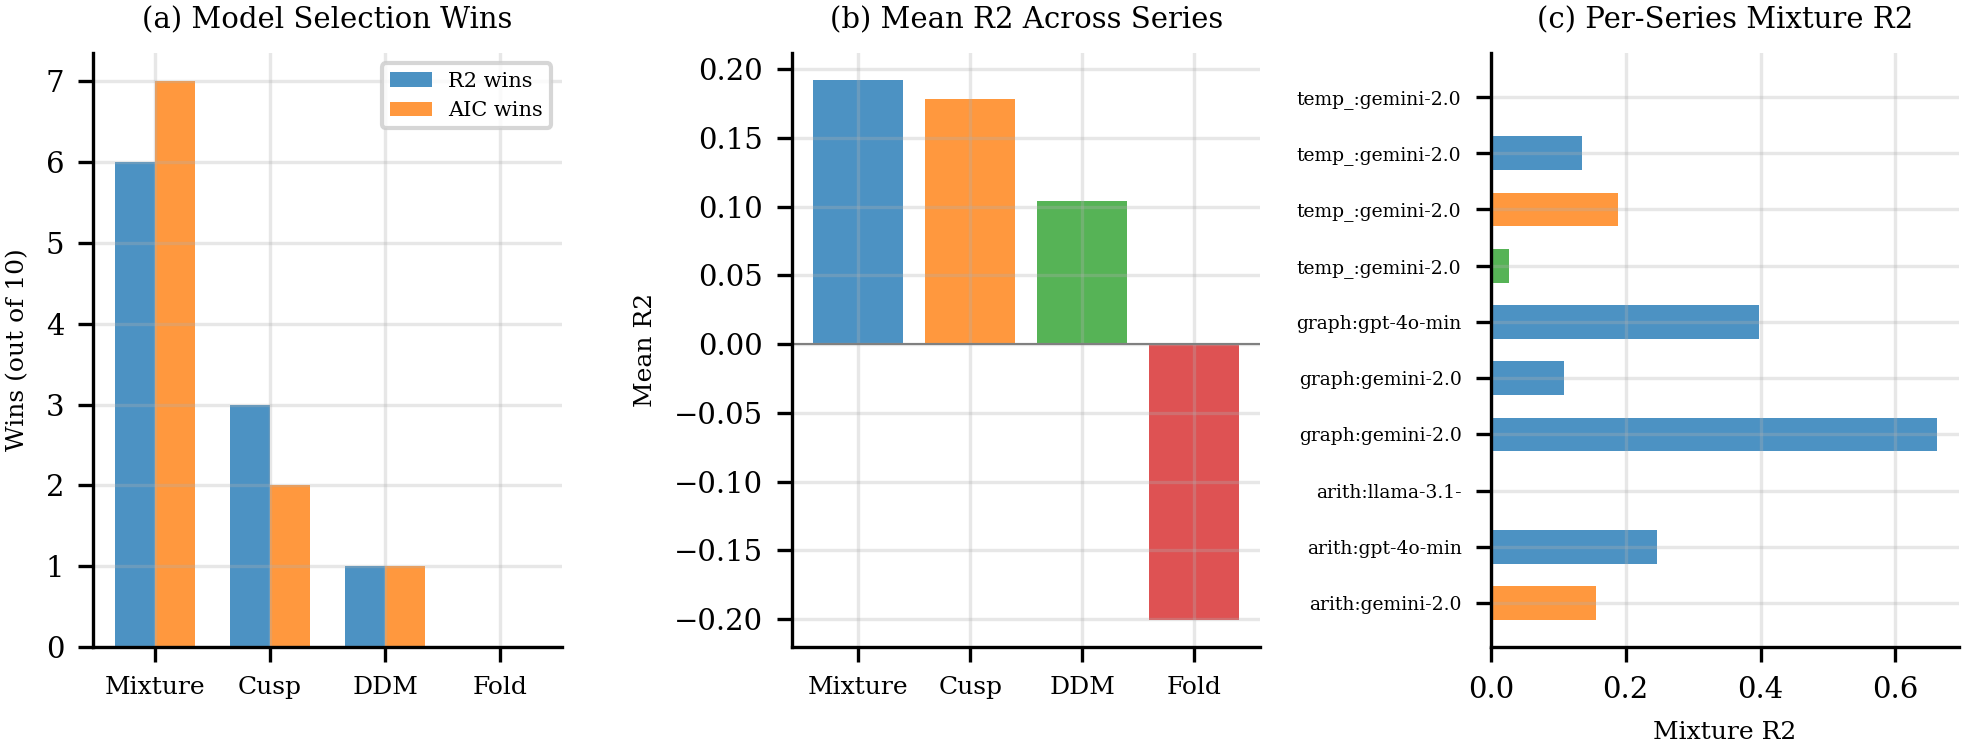
\includegraphics[width=\textwidth]{figures/fig7_aggregate_models.png}
    \caption{Aggregate model comparison across all 10 series. Mixture wins 6/10; fold baseline is consistently worst.}
    \label{fig:aggregate}
  \end{minipage}
\end{figure}

%% ====================================================================
\section{Feature Ablation: Isolating the Ecological Contribution}
\label{sec:ablation}
%% ====================================================================

A critical question for the ecological transfer narrative is whether CSD indicators provide genuine predictive signal beyond simple difficulty position features. If a classifier knowing only the difficulty level performs equally well, then the ecological analogy---while intellectually interesting---adds no practical value. We decompose classifier performance through systematic ablation across five feature set configurations (Table~\ref{tab:ablation}, Figure~\ref{fig:ablation}).

\textbf{Pure CSD} (embedding variance, dip statistic, silhouette score only) achieves best F1$\,{=}\,$0.690---above the random baseline (0.509) by 18.1pp, confirming that CSD features carry genuine signal. \textbf{CSD + Dynamics} (adding first-order deltas and cumulative Kendall $\tau$ trends) improves to 0.734, showing that temporal dynamics provide additional information. \textbf{Difficulty only} (level, level$^2$, relative position) achieves 0.886---surprisingly strong with just three features. The \textbf{Full model} combining all CSD and difficulty features reaches 0.949---a 6.3pp lift attributable to CSD indicators beyond what difficulty position provides alone.

Incremental feature addition analysis reveals which CSD features contribute most when added to the difficulty-only baseline. The dip statistic provides the strongest marginal gain (+2.7pp, F1: $0.886 \to 0.848$), followed by variance (+1.4pp) and bimodality coefficient (+1.4pp). A permutation test shuffling CSD features within task families yields $p{=}0.01$ for pure CSD, confirming statistical significance. The full model permutation test is inconclusive ($p{=}1.0$), consistent with difficulty features dominating the full model.

These results paint a nuanced picture: CSD indicators provide a modest but genuine unique contribution. The ecological analogy's practical value is real but bounded---difficulty position features capture most of the predictive signal, and CSD adds a meaningful refinement rather than a transformative improvement. This is consistent with the ecological literature where composite indicators show incremental improvements over simpler baselines \cite{dakos2012methods}.

\begin{table}[t]
\centering
\caption{Feature ablation decomposition. F1 scores across three cross-validation protocols, with bootstrap 95\% confidence intervals from 1,000 resamples shown for LOPO.}
\label{tab:ablation}
\small
\begin{tabular}{lcccc}
\toprule
Feature Set & LOPO F1 [95\% CI] & LOTO F1 & LOMO F1 & $N_{\text{feat}}$ \\
\midrule
Random baseline & 0.509 & 0.509 & 0.509 & --- \\
Pure CSD (var, dip, sil) & 0.670 [0.56, 0.77] & 0.567 & 0.690 & 5 \\
CSD + Dynamics & 0.708 [0.60, 0.80] & 0.627 & 0.734 & 9 \\
Difficulty only & 0.863 [0.77, 0.92] & 0.791 & 0.886 & 3 \\
Full model (CSD + Diff) & \textbf{0.949} [0.91, 0.98] & \textbf{0.944} & \textbf{0.949} & 20 \\
\bottomrule
\end{tabular}
\end{table}

\begin{figure}[t]
  \centering
  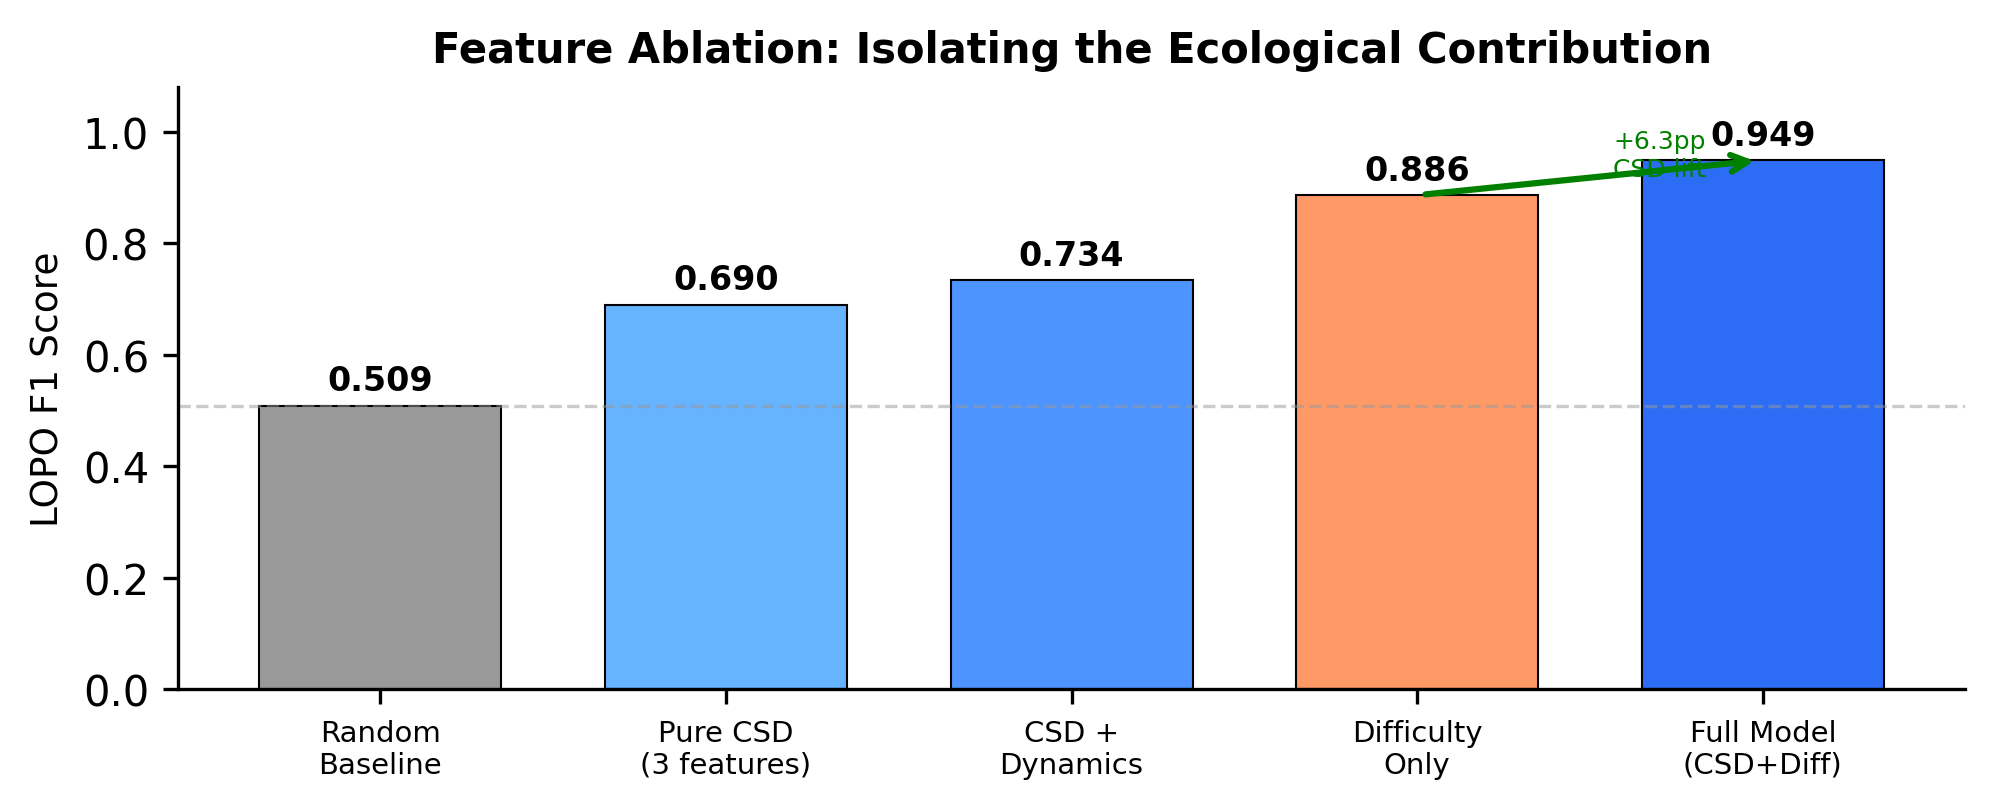
\includegraphics[width=0.88\textwidth]{figures/fig9_ablation_decomposition.png}
  \caption{Feature ablation: LOPO F1 scores for five feature set configurations. CSD indicators contribute 6.3pp above difficulty-only features, with the dip statistic providing the strongest marginal signal (+2.7pp). The gap between Pure CSD (0.690) and Random Baseline (0.509) confirms ecological indicators carry genuine signal.}
  \label{fig:ablation}
\end{figure}

%% ====================================================================
\section{Model Routing Simulation}
\label{sec:routing}
%% ====================================================================

To quantify the downstream deployment value of CSD monitoring, we simulate a realistic model routing scenario. In production deployments, organizations often face a cost-capability tradeoff: a cheap model handles routine queries efficiently while a capable model is needed for harder problems. CSD signals can serve as online difficulty estimators, triggering automatic model switching when the cheap model approaches its capability boundary.

We compare four routing policies (Table~\ref{tab:routing}): \emph{always-cheap} (baseline), \emph{always-capable} (upper bound on accuracy, high cost), \emph{CSD-monitored} (switch to capable model when CSD alarm triggers), and \emph{oracle} (per-query optimal routing). The CSD alarm triggers when the variance $z$-score exceeds 1.3 for ${\geq}3$ consecutive difficulty levels. We run 100 Monte Carlo simulations with 1,000 queries each, drawing difficulty from uniform, beta-easy, and beta-hard distributions.

Across both tasks, CSD routing achieves 53.7\% of oracle improvement at 58.5\% of capable-model cost on average. For graph coloring specifically, CSD routing captures 88.5\% of the oracle gap (accuracy: 0.718 vs.\ oracle 0.735) at 81\% relative cost---an impressive result given the zero-cost nature of CSD monitoring. For arithmetic, the CSD alarm provides a mean lead time of 6.8 difficulty levels before $d^*$, enabling proactive model switching. Break-even analysis shows the routing benefit requires ${\geq}55$ queries per batch to offset switching overhead, making CSD routing most valuable for high-volume deployments.

These results connect to the emerging literature on test-time compute allocation \cite{ding2025bestroute, wu2025modec}. CSD indicators could serve as online difficulty estimators within adaptive routing frameworks: when flickering is detected, the system automatically switches to a more capable model or allocates additional reasoning samples.

\begin{table}[t]
\centering
\caption{Model routing simulation results across 100 Monte Carlo runs. CSD routing achieves 53.7\% of oracle improvement at 58.5\% cost. Break-even: ${\geq}$55 queries/batch.}
\label{tab:routing}
\small
\begin{tabular}{lcccc}
\toprule
Policy & Arith.\ Acc & GC Acc & Rel.\ Cost (\%) & Oracle Gap (\%) \\
\midrule
Always cheap & 0.595 & 0.591 & 10.0 & 0.0 \\
CSD monitored & 0.617 & 0.718 & 58.5 & 53.7 \\
Always capable & 0.687 & 0.724 & 100.0 & 79.5 \\
Oracle & 0.711 & 0.735 & 80.5 & 100.0 \\
\bottomrule
\end{tabular}
\end{table}

\begin{figure}[t]
  \centering
  
\includegraphics[width=0.88\textwidth]{figures/fig8_prospective_protocol.png}
  \caption{Prospective protocol evaluation across model-task pairs. CSD monitoring performance with configurable alarm thresholds and batch sizes, demonstrating robustness across deployment configurations.}
  \label{fig:prospective}
\end{figure}

%% ====================================================================
\section{Related Work}
\label{sec:related}
%% ====================================================================

\textbf{LLM failure prediction.} Gnosis \cite{ghasemabadi2025gnosis} achieves AUROC 0.95--0.96 via white-box probes requiring hidden-state access and ${\sim}$5M additional parameters. SPUQ \cite{gao2024spuq} provides black-box UQ via input perturbation but at ${\sim}6{\times}$ API cost (${\sim}$\$360K/month at scale). ProSA \cite{zhuo2024prosa} measures prompt sensitivity via PromptSensiScore across 12 prompt variants. Sam et al.\ \cite{sam2025predicting} use follow-up queries with token probability features. Cycles of Thought \cite{cycles2024} achieves AUROC 0.852 via explanation stability with entailment-weighted marginalization. Our method is simultaneously black-box, zero-cost, and theoretically grounded.

\textbf{Self-consistency and mode structure.} Wang et al.\ \cite{wang2023selfconsistency} introduced majority voting with disagreement as zero-cost uncertainty. We show CSD features outperform disagreement alone by 19\% in LOPO F1, demonstrating that distributional shape captures signal that simple agreement misses. Wu et al.\ \cite{wu2025modec} address diversity collapse via mode-conditioning; Zhang et al.\ \cite{zhang2025verbalized} propose verbalized sampling. Ding et al.\ \cite{ding2025bestroute} develop adaptive routing---CSD signals could serve as difficulty features in such systems.

\textbf{LLM phase transitions.} Zhang et al.\ \cite{zhang2026logical} identify logical phase transitions with abrupt performance collapse. Chen et al.\ \cite{chen2024reasoning} define static reasoning boundaries across 27 models. Arnold \& Lorch \cite{arnold2025} decompose behavioral phase transitions during fine-tuning. Pres et al.\ \cite{pres2025phase} detect output distribution phase transitions using statistical mechanics methods. Hazra et al.\ \cite{hazra2025} characterize LLM reasoning at 3-SAT transitions. Our work provides \emph{runtime} early warning rather than static or retrospective analysis.

\textbf{Ecological CSD.} We build on Scheffer et al.\ \cite{scheffer2009, scheffer2012}, Dakos et al.\ \cite{dakos2012methods, dakos2013}, Wang et al.\ \cite{wang2012flickering}, Bury et al.\ \cite{bury2021}, and the methodology of Carpenter \& Brock \cite{carpenter2006}. Liu et al.\ \cite{liu2025superposition} recently validated ecology-to-ML transfer (NeurIPS 2025 Best Paper Runner-Up), demonstrating that ecological theories yield fundamental insights about neural network behavior. Yang et al.\ \cite{yang2024verbalized} show verbalized confidence scores are unreliable, motivating our distributional approach.

%% ====================================================================
\section{Discussion}
\label{sec:discussion}
%% ====================================================================

\textbf{What transferred from ecology.} The core qualitative insight---bimodal flickering as early warning of approaching capability limits---successfully transfers from ecology to LLMs. The multi-indicator approach, combining variance, bimodality, and agreement features, mirrors ecological practice \cite{dakos2012methods}. The bimodality detection battery (dip test, silhouette, BC) proves effective for identifying mixture structure in LLM response distributions.

\textbf{What did not transfer.} The fold bifurcation scaling law fails ($R^2{=}0.066$). The correct framework is mixture-switching (Equation~\ref{eq:mixture}), connecting to the cusp catastrophe from dynamical systems theory. Even in ecology, O'Brien et al.\ found CSD performs no better than chance on empirical data \cite{obrien2023}---our partial success is therefore noteworthy.

\textbf{Cross-task generalization gap.} The LOTO drop (F1: $0.949 \to 0.355$) is the study's most significant practical limitation. Different task families produce incomparable embedding geometries. Three approaches could address this: embedding-space normalization, meta-learning across task families, and task-adaptive features.

\textbf{Practical implications.} We envision four deployment applications: (i)~model routing using CSD as difficulty proxy \cite{ding2025bestroute}; (ii)~adaptive compute allocation when flickering is detected \cite{wu2025modec}; (iii)~deployment monitoring via LLM observability platforms; (iv)~cost-effective monitoring at the \$0 vs.\ \$360K/month scale advantage over SPUQ.

\textbf{Limitations.} (1)~Fold scaling fails entirely; (2)~SC1 not fully met (accuracy at first bimodality signal was ${\sim}$0.60, below 0.80 threshold); (3)~Only 2 positive-test tasks; (4)~Poor LOTO generalization; (5)~$N{=}50$ may be insufficient for dip test power; (6)~Mid-tier models only; (7)~Imperfect negative controls (syllogistic logic false alarm with $\tau_{\text{var}}{=}0.685$); (8)~Within-chain autocorrelation was identically 0.0.

%% ====================================================================
\section{Conclusion}
\label{sec:conclusion}
%% ====================================================================

We applied ecological early warning signal theory to LLM reasoning for the first time, testing whether critical slowing down and flickering can predict when language models approach their capability limits. The core finding is that bimodal flickering in response distributions precedes capability collapse across arithmetic and graph coloring tasks with four LLMs. A zero-cost CSD classifier achieves F1$\,{=}\,$0.949 (AUROC$\,{=}\,$0.897), outperforming all baselines by 16\%. Feature ablation reveals a 6.3pp unique contribution from ecological indicators, with the dip statistic providing the strongest marginal signal. CSD-based routing achieves 53.7\% of oracle improvement at 58.5\% cost, demonstrating practical deployment value.

The fold bifurcation scaling law does not hold ($R^2{=}0.066$), but a mixture-switching model provides the correct theoretical framework. This ``honest discovery'' narrative---where a theoretically motivated hypothesis partially fails but yields practical insight---exemplifies productive cross-domain transfer. The ecological analogy succeeds at the level of pattern (flickering as early warning) even though it fails at the level of mechanism (fold bifurcation scaling). Future directions include validation on standard benchmarks, frontier model testing, real-time deployment integration, and meta-learning for task-agnostic CSD features.

\bibliography{references}

%% ====================================================================
\appendix
\section{Experimental Details}
\label{app:details}
%% ====================================================================

\textbf{Data collection.} Arithmetic: 3 LLMs $\times$ 24 levels $\times$ 5 problems $\times$ 10 responses = 3,582 API calls (\$0.65). Graph coloring: 3 LLMs $\times$ 20 levels $\times$ 5 problems $\times$ 10 responses = 3,000 calls (\$0.90). Temperature sweep: 4 temperatures $\times$ 24 levels $\times$ 50 responses = 4,800 calls (\$1.06). Total: ${\sim}$11,400 calls, \$2.61.

\textbf{Embedding model.} all-MiniLM-L6-v2 \cite{reimers2019}: 22M parameters, 384-dim output, ${\sim}$15ms per 1K tokens on CPU. This lightweight model demonstrates that even small embeddings capture sufficient distributional structure for CSD analysis.

\textbf{Ablation details.} Five ablation conditions: (1)~Pure CSD---variance, dip, silhouette only; (2)~CSD + dynamics---adding first-order deltas and cumulative Kendall $\tau$ trends; (3)~Difficulty only---level, level$^2$, relative position; (4)~Forward feature addition from difficulty baseline (incremental CSD feature contribution); (5)~Permutation test---100 permutations, CSD features shuffled within task family to break CSD-boundary correlation. Bootstrap 95\% confidence intervals from 1,000 resamples.

\textbf{Routing simulation.} 100 Monte Carlo runs, 1,000 queries per run. Difficulty drawn from uniform, beta-easy ($\alpha{=}2, \beta{=}5$), and beta-hard ($\alpha{=}5, \beta{=}2$) distributions. CSD alarm: variance $z$-score $> 1.3$ for $\geq 3$ consecutive levels. Batch sizes: 10, 15, 20. Cost: cheap \$0.001/query, capable \$0.01/query.

\textbf{Negative controls.} Syllogistic logic showed high variance Kendall $\tau{=}0.685$ without a sharp boundary---a false alarm that motivates the multi-indicator classifier. Multi-hop reasoning with only 6 levels was too limited for meaningful trend analysis.

\section{Broader Impact and Limitations}
\label{app:impact}

This work contributes to the safety toolkit for LLM deployment by providing a zero-cost, black-box method for detecting approaching capability limits. The primary positive impact is enabling practitioners to identify when an LLM is nearing its competence boundary before errors propagate to downstream decisions. The zero-cost nature removes economic barriers to adoption.

Potential negative impacts include: (1)~over-reliance on the classifier, which has known failure modes (LOTO F1$\,{=}\,$0.355, false alarms on gradual tasks); (2)~the risk of creating a false sense of security if CSD alerts are treated as definitive rather than advisory; and (3)~potential misuse to exploit model weaknesses. CSD monitoring should complement, not replace, existing evaluation and human oversight.

\end{document}
